%% Estructura principal para un reporte de Trabajos intersemanales CIRCAE %%
\documentclass[a4paper]{IEEEtran} %tamaño del papel y el tipo de transcripción que será IEEE
\usepackage[utf8]{inputenc} %el tipo de codificación que incluye símbolos como la tilde
\usepackage[spanish]{babel} % hacemos que nuestro documentación vaya en español
\usepackage{cite} % citas bibliográficas
\usepackage{graphicx} %gráficos, usaremos solo .jpg o .png con estándares que ya veremos
\usepackage{subfigure}
\usepackage{url}
\usepackage{amsmath}
\usepackage{booktabs} 
\providecommand{\keywords}[1]{\textbf{\textit{Términos Clave---}} #1}
\begin{document}
%\tableofcontents%tabla de contenidos
%\listoffigures%lista de figuras
\title{Control De Posición De Brazo Levitado Por Hélice}
\author{Champi Castro Miguel Angel, Quispe Condori Hanan Ronaldo, Sevilla Hidalgo Alfonso Alejandro}
\markboth{Teoría de Control I 2019-11-16}{} % Codigo del informe que corresponde a: semestre | mes | dia | numero de grupo con la G antepuesta | numero de proyecto con la P antepuesta | número de informe
\maketitle
\begin{abstract}
En este proyecto implementaremos el control de un brazo levitado por hélice, esto se logrará modificando la velocidad de giro de la hélice con el fin de que el brazo se encuentre en una posición deseada.
\end{abstract}
\section{Modelamiento Matemático}
\label{sec:modelamiento}
El modelamiento de este sistema tendra dos partes, en la primera parte modelaremos el subsistema mecánico del brazo y en la segunda parte el subsistema motor-hélice \cite{gunel2016modeling}.
\begin{figure}[h]
    \centering
        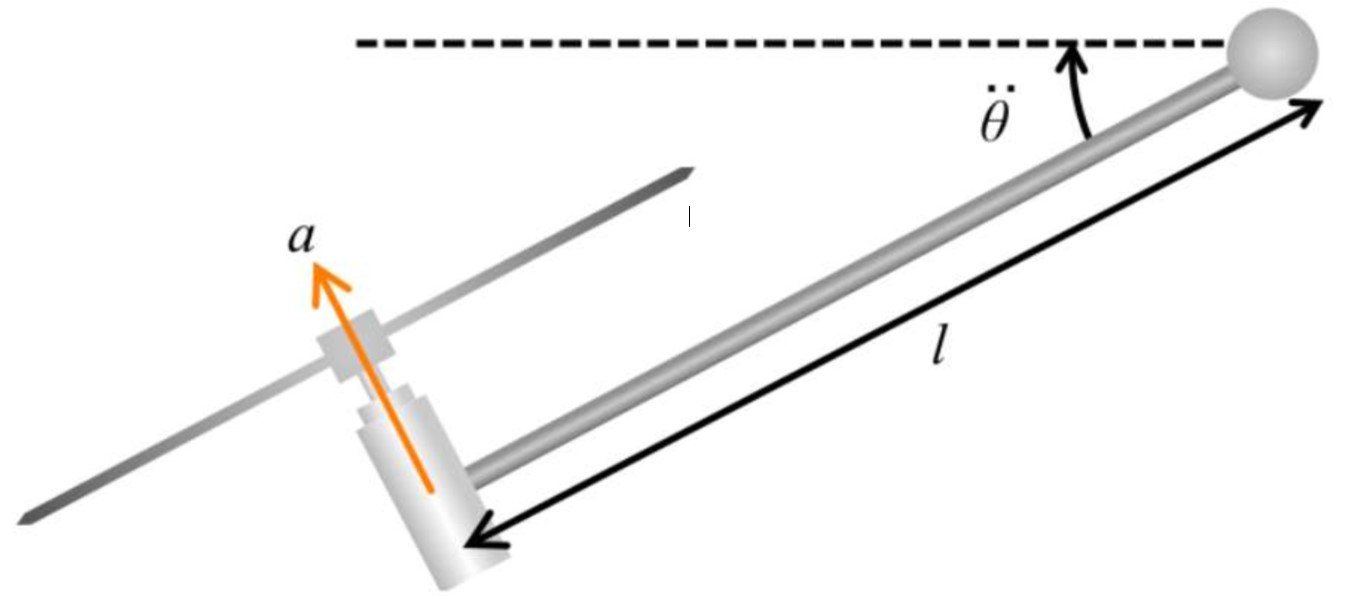
\includegraphics[width=8cm]{images/1}
        \caption{Diagrama del Sistema Completo.}
        \label{fig:DLC}
\end{figure}

Haciendo uso del diagrama de cuerpo libre, ecauciones difreenciales y la transformada de Laplace para el calculo de la función de transferencia. 

En el subsistema del motor-hélice tendremos.
%Ecuación del motor. 
\begin{equation}
    \begin{split}
        V_{s}&=R_{i}+L\frac{di}{dt}+e_{t}\\
        e_{t}&=k_{f}\frac{d\theta}{dt}\\
    \end{split}
    \label{eq:motor}
\end{equation}
Torque en hélice
\begin{equation}
    \begin{split}
        T_{l}&=J_{p}\frac{d^2\theta}{dt^2}\\
    \end{split}
    \label{eq:helix}
\end{equation}
En el torque en el motor tendremos
\begin{equation}
    \begin{split}
        T_{r}&=J_{1}\frac{d^2\theta}{dt^2}+B\frac{d\theta}{dt}+T_{l}\\
        T_{r}&=k_{t}i(t)\\
        k_{t}i(t)&=J_{1}\frac{d^2\theta}{dt^2}+B\frac{d\theta}{dt}+J_{p}\frac{d^2\theta}{dt^2}\\
    \end{split}
        \label{eq:motortork}
\end{equation}
En el dominio de Laplace tendremos
\begin{equation}
    \begin{split}
        I(s)&=\frac{(J_{1}+J_{p})s^2 +Bs}{k_{t}}\theta(s)\\
    \end{split}
    \label{eq:laplas}
\end{equation}
Torque en el subsistema del brazo, sustituyendo \ref{eq:helix} tendremos.
\begin{equation}
    \begin{split}
        T_{l}&=J_{B}\frac{d^2\theta_{B}}{dt^2}\\
        J_{p}\frac{d^2\theta}{dt^2}&=J_{B}\frac{d^2\theta_{B}}{dt^2}\\
    \end{split}
    \label{eq:torkbrazo}
\end{equation}
LLevando \ref{eq:torkbrazo} al dominio de Laplace 
\begin{equation}
    \begin{split}
        \theta(s)&=\frac{J_{B}}{J_{p}}\theta_{B}(s)\\
    \end{split}
    \label{eq:torkbrazoplace}
\end{equation}
LLevando \ref{eq:motortork} al dominio de Laplace 
\begin{equation}
    \begin{split}
        V_{s}(s)&=RI(s)+LSI(s)+k_{f}S\theta(s)\\
        V_{s}(s)&=k_{f}S\theta(s)+(R+LS)\frac{(J_{1}+J_{p})S^2+BS}{k_{t}}\theta(s)\\
        V_{s}(s)&=\frac{k_{f}k_{t}S+(R+LS)((J_{1}+J_{p})S^2+BS)}{k_{t}}\theta(s)\\
    \end{split}
    \label{eq:motorenplace}
\end{equation}
Reemplazando \ref{eq:torkbrazoplace} en \ref{eq:motorenplace} tendremos la función de transferencia$$F(s)$$.
\begin{equation}
    \begin{split}
        \frac{k_{t}J_{p}}{(k_{f}+k_{t})LS^3J_{B}+J_{B}S^2(LB+R(J_{1}+J_{p}))+S(RB+k_{f}k_{t})}\\
    \end{split}
    \label{eq:transfer}
\end{equation}
%\vspace{5mm}

\section{Espacio de Estados}
Apartir de la funcion de transferencia hallada en la seccion anterior podremos calcular lo siguiente.

Considerando
\begin{equation}
    \begin{split}
        A&=J_{B}L(J_{p}+J_{1})\\
        B&=J_{B}(LB+R(J_{p}+J_{1}))\\
        C&=J_{B}(RB+k_{f}k_{t})\\
        D&=J_{p}k_{t}\\
    \end{split}
    \label{eq:consideraciones}
\end{equation}
Reemplazando \ref{eq:consideraciones} en \ref{eq:transfer} la función de transferencia queda de la siguiente manera.
\begin{equation}
    \begin{split}
        \theta_{B}(s)[AS^3+BS^2+CS]&=DV_{s}(s)\\
        A\ddot{\theta_{B}}+B\ddot{\theta_{B}}+C\dot{\theta_{B}}&=DV_{s}(s)\\
        A\ddot{\theta_{B}}&=DV_{s}-B\ddot{\theta_{B}}-C\dot{\theta_{B}}\\
    \end{split}
    \label{eq:consideraciones}
\end{equation}
%\vspace{10mm}
\bibliographystyle{ieeetr}
\bibliography{bibliografia}
\end{document}